\documentclass[12pt,a4paper,parskip=full]{scrartcl}

\usepackage{bbding}
\usepackage{pifont}
\usepackage{wasysym}
\usepackage[margin=1in]{geometry}
\geometry{letterpaper}
\usepackage{xcolor}
\definecolor{red}{HTML}{cc0000}
\definecolor{gray}{HTML}{666666}
\usepackage{sectsty}
\sectionfont{\color{red}}
\subsectionfont{\color{red}}
\usepackage[dvipdfmx]{graphicx}
%\usepackage{graphicx}
\usepackage{hyperref}
\usepackage{amssymb}
\usepackage[style=footnote-dw]{biblatex}
\bibliography{S@SGuideBib}
\setlength\bibitemsep{0.5\baselineskip}

\usepackage{enumitem}
\setitemize{noitemsep}
% \setlist{noitemsep, topsep=-5pt}
% \setlength\itemsep{-0.10em}

\renewcommand{\labelitemi}{$\cdot$}
\renewcommand{\labelitemii}{$\cdot$}
\makeatletter
\let\latexl@section\l@section
\def\l@section#1#2{\begingroup\let\numberline\@gobble\latexl@section{#1}{#2}\endgroup}
\makeatother

\usepackage[T1]{fontenc}
\fontfamily{verdana}

\usepackage{scrlayer-scrpage}{}
\makeatletter
\renewcommand{\@seccntformat}[1]{}
\makeatother

\setlength\parindent{0pt}{}

\title{\Huge{\color{red}\textbf{The Scrum@Scale
\textsuperscript{\copyright}
Guide}}}
\subtitle{\color{gray}The Definitive Guide to Scrum@Scale:\\ Scaling that
Works}
% \author{}
\date{}


\begin{document}

%\tableofcontents
%\newpage

\if0
\section{Purpose of the Scrum@Scale Guide}
\fi
\section{Scrum@Scaleガイドの目的}
\if0
Scrum, as originally outlined in the Scrum Guide, is a framework for
developing, delivering, and sustaining complex products by a single team.
Since its inception, its usage has extended to the creation of products,
processes, services, and systems that require the efforts of multiple
teams. Scrum@Scale was created to efficiently coordinate this new ecosystem
of teams in a way that optimizes the overall strategy of the organization.
It achieves this goal through setting up a ``minimum viable bureaucracy''
via a scale-free architecture, which naturally extends the way a single
Scrum team functions across the organization.
\fi
スクラムは、もともとスクラムガイドで概説されているように、単一のチームに
よって複雑なプロダクトを開発、提供、および維持することができる。
発行以来、複数チームの協力が求められる、プロダクト、プロセス、サービス、システム
などの開発にまで広がりを見せている。
Scrum@Scaleは、組織戦略の全体を最適化する方法として、チームの新しいエコシ
ステムを効率的に調整するために作成された。
これは、単一スクラムチームを、組織で機能横断的に自然に拡張するというスケー
ルフリーなアーキテクチャにより、``最小で実行可能な官僚制''の導入を通じて
目的を達成するものである。

\if0
This guide contains the definitions of the components that make up the
Scrum@Scale framework, including its scaled roles, scaled events, and
enterprise artifacts, as well as the rules that bind them together.
\fi
このガイドには、Scrum@Scale フレームワーク、スケール化ルール、スケール化イベント、
といったコンポーネントの定義と、エンタープライズ向け成果物、およびそれらを結び
つけるルールが含まれている。

\if0
Dr. Jeff Sutherland developed Scrum@Scale based on the fundamental
principles behind Scrum, Complex Adaptive Systems theory, game theory, and
object-oriented technology. This guide was developed with the input of many
experienced Scrum practitioners based on the results of their field work.
The goal of this guide is for the reader to be able to implement Scrum@Scale
on their own.
\fi
ジェフ・サザーランド博士は、スクラムの背後にある原則、複雑な適応システム理論、
ゲーム理論、オブジェクト指向技術に基づきScrum@Scaleを開発した。
このガイドは、多くの経験豊かなスクラムの実践者のフィールドワークの結果に基づい
て開発されている。
このガイドは、読者が自分自身でScrum@Scaleを実践できることを目的としている。

\if0
\subsection{Why Scrum@Scale?}
\fi
\subsection{なぜScrum@Scaleか?}
\if0
Scrum was designed for a single team to be able to work at its optimal
capacity while maintaining a sustainable pace. In the field, it was found
that as the number of Scrum teams within an organization grew, the 
output (working product) and velocity of those teams began to fall (due to
issues like cross-team dependencies and duplication of work). It became
obvious that a framework for effectively coordinating those teams was
needed in order to achieve linear scalability. Scrum@Scale is designed to
accomplish this goal via its scale-free architecture.
\fi
スクラムは、単一のチームが持続可能なペースを維持し、その最適な能力で働く
ことができるようにデザインされている。
現場では、組織内のスクラムチーム数の増加に伴いアウトプット(プロダクト)とベロ
シティの低下が見受けられる(冗長な作業やチーム横断依存のような問題のため)。
リニアなスケーラビリティを得るためには、複数のチームを効果的に調整するための
フレームワークが必要であることが明白である。
Scrum@Scaleは、スケールフリーアーキテクチャで目的を達成するためにデザイン
されている。

\if0
By utilizing a scale-free architecture, the organization is not constrained
to grow in a particular way determined by a set of arbitrary rules; rather
it can grow organically based on its unique needs and at a sustainable pace
of change that can be accepted by the groups of individuals that make up
the organization. The simplicity of the Scrum@Scale model is essential to a scale-free architecture and carefully avoids introducing extra complexity that will cause productivity per team to decrease as more teams are created.
\fi
スケールフリーアーキテクチャを利用することによって、組織は成長するための特定
の方法に任意の規則のセットの決定や方法を強制されない。
むしろ、それは、そのユニークなニーズ、および組織を作る個人のグループにより受け
入れられうる変化の持続可能なペースに有機的に基づくかもしれない。
Scrum@Scaleモデルのシンプルさはスケールフリーアーキテクチャに必須で、チーム
あたり生産性を、より多くのチームが作成されると減少させる特別な複雑さを導入する
ことを慎重に避ける。

\if0
Scrum@Scale is designed to scale across the organization as a whole: all
departments, products and services. It can be applied across multiple
domains in all types of organizations in industry, government, or academia.
\fi
Scrum@Scaleは、すべての部門、プロダクト、およびサービスといった、組織全体を横断的に
スケールするようにデザインされている。
それは、産業、政府、または学界の組織のすべてのタイプの複数定義域を横断的に適
用できる。

\if0
\subsection{Definition of Scrum@Scale}
\fi
\subsection{Scrum@Scaleの定義}
\if0
Scrum: A framework within which people can address complex adaptive
problems, while productively and creatively delivering viable products of the
highest possible value.
\fi
スクラム: 現実的で高価値のプロダクトを生産性と創造性をもってデリバリするため、
複雑な問題への順応的対処に取り組むことができるフレームワーク。

\if0
The Scrum Guide is the minimal feature set that allows inspection and
adaptability via radical transparency to drive innovation, customer satisfaction, performance, and
team happiness.
\fi
スクラムガイドは、根本的な透明性をもった検査と適応性が、革新、顧客満足、性能、
およびチーム幸福を駆動するという、最小のフィーチャーセットである。

\if0
Scrum@Scale: A framework within which networks of Scrum teams operating
consistently with the Scrum Guide can address complex adaptive problems,
while creatively delivering products of the highest possible value.
\fi
Scrum@Scale: 現実的で高価値のプロダクトを創造的にデリバリするため、
複雑な問題への順応的対処に取り組むことができるスクラムガイドとともに、
複数スクラムチームが一貫して機能するネットワーク内のフレームワーク。

\if0
\textbf{NOTE:} These ``products'' may be hardware, software, complex
integrated systems, processes, services, etc., depending upon the domain of
the Scrum teams.
\fi
\textbf{注意:} これら ``プロダクト'' は、スクラムチームのドメインに応じて、ハードウェア、
ソフトウェア、複雑に統合されたシステム、プロセス、サービスなどであるかもしれない。

\if0
Scrum@Scale is:
\begin{itemize}
\item Lightweight - the minimum viable bureaucracy
\item Simple to understand - consists of only Scrum teams
\item Difficult to master - requires implementing a new operating model
\end{itemize}
\fi
Scrum@Scale とは:
\begin{itemize}
\item 軽量 - 最小で実行可能な官僚制
\item 理解しやすい - スクラムチームだけから成る
\item 習得は難しい - 新しい運用モデルを身に着ける必要がある
\end{itemize}


\if0
Scrum@Scale is a framework for scaling Scrum. It radically simplifies
scaling by using Scrum to scale Scrum. 
\fi
Scrum@Scaleは、スクラムをスケールするためのフレームワークである。
それは、スクラムをスケールするために、スクラムを使用してスケールすることを
抜本的に簡素化する。

\if0
In Scrum, care is taken to separate accountability of the ``what'' from the
``how''. The same care is taken in Scrum@Scale so that jurisdiction and
accountability are expressly understood in order to eliminate wasteful
organizational conflict that keep teams from achieving their optimal
productivity.
\fi
スクラムでは、``How''と``What'' の責任の分離に注意する必要がある。
Scrum@Scaleでも同様に、チームの最適な生産性を達成を邪魔する、無駄な
組織上の衝突を取り除くために、権限と責務を明確に理解し、注意する必要がある。

\if0
Scrum@Scale consists of components that allow an organization to
customize their transformational strategy and implementation. It gives them
the ability to target their incrementally prioritized change efforts in the area(s) they deem
most valuable or most in need of change and then progress on to others.
\fi
Scrum@Scaleは、組織変革の戦略とインプリメンテーションをカスタマイズ
することを可能にするコンポーネントから成る。
それらは、彼らが最も重要であると判断した領域、または変更の必要性が最も高い領域で
段階的に優先順位を付けた変更の取り組みを目標とし、順次進んでいく能力を与える。

\if0
In separating these two jurisdictions, Scrum@Scale contains two cycles: the
Scrum Master Cycle (the ``how'') and the Product Owner Cycle (the
``what''), each touching the other at two points. Taken together, these
cycles produce a powerful framework for coordinating the efforts of
multiple teams along a single path.
\fi
これら2つの権限を分離されており、Scrum@Scaleは、2つのサイクルを含んでいる:
スクラムマスターサイクル(``How'')、およびプロダクトオーナーサイクル
(``What'')であり、2つポイントで接触する。
まとめると、これらのサイクルは、一直線上に複数のチームの取り組みを調整するための
強力なフレームワークを作り出す。

\if0
\subsection{The Components of the Scrum@Scale\textregistered ~Framework}
\fi
\subsection{Scrum@Scaleの構成要素\textregistered ~フレームワーク}

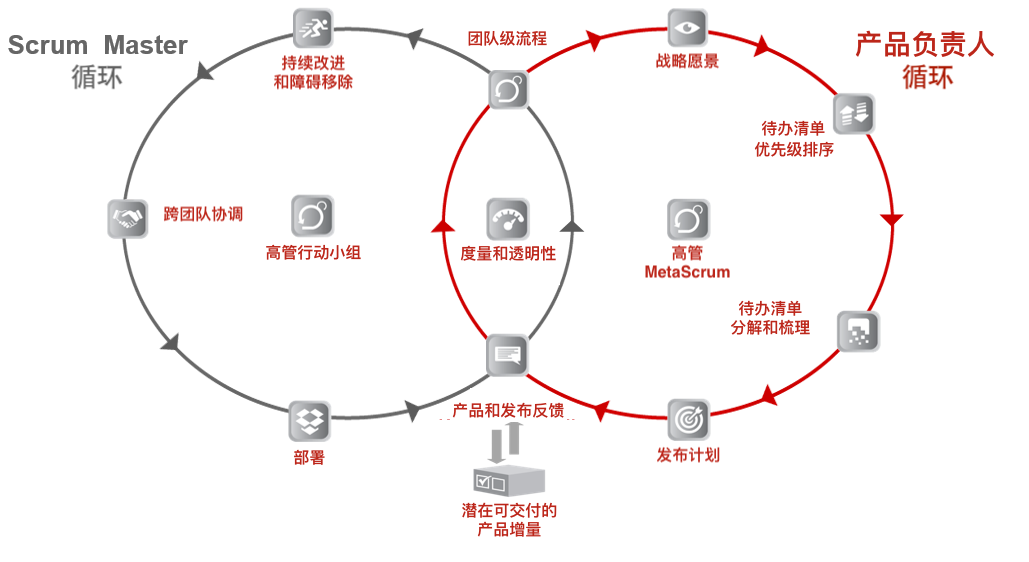
\includegraphics[width=1.0\linewidth]{SMPO-Cycle.png}

\if0
\subsection{Values-Driven Culture}
\fi
\subsection{価値駆動文化}
\if0
Besides separating accountability of the ``what'' and the ``how,''
Scrum@Scale further aims to build healthy organizations by creating a
values-driven culture in an empirical setting. The Scrum values are:
Openness, Courage, Focus, Respect, and Commitment. These values drive
empirical decision making, which depend on the three pillars of
transparency, inspection, and adaptation.
\fi
``What'' および``How''の責務の分離以外では、Scrum@Scaleは、
実証的な環境で価値駆動文化を創り出すことで、健全な組織を構築することを
さらなる目的としている。スクラムにおける価値とは次のようなものがある: 
オープン性、勇気、集中、敬意、コミットメント。これらの価値が、経験的意思決定を促進する。
それは、透明性、検査、および適応の3つの柱により成り立っている。

\if0
Openness supports transparency into all of the work and processes, without
which there is no ability to inspect them honestly and attempt to adapt
them for the better. Courage refers to taking the bold leaps required to
deliver value quicker in innovative ways.
\fi
オープン性は、すべての作業とプロセスへの透明性を保証する。
さもなくば誠実な検査と、より良いものに適合していくことはできない。
勇気は、革新的な方法で、より迅速な価値をデリバリするために必要な、大胆な飛躍する
ことを示す。

\if0
Focus and Commitment refer to the way we handle our work obligations,
putting customer value delivery as the highest priority. Lastly, all of
this must occur in an environment based on respect for the individuals
doing the work, without whom nothing can be created.
\fi
集中とコミットメントは、自分たちで自分たちの責務を全うする方法を見つけることを示し、
顧客へ価値を届けることを最優先とするということである。
最後に、これらすべては、他のだれも成しえないことを行っている作業者個人
個人へのリスペクトに支えられた環境なくしては成しえない。

\if0
Scrum@Scale helps organizations thrive by supporting a
transformational leadership model which fosters a positive environment for
working at a sustainable pace and putting commitment to deliver
customer-facing value at the forefront of our efforts.
\fi
Scrum@Scaleは、持続可能なペースで働くための積極的な環境を育て、
努力の最前線で顧客が直面する価値を届けるというコミットメントをもたらす、
変革リーダーシップモデルをサポートすることによって、組織の成長を支援する。

\if0
\subsection{Getting Started with Scrum@Scale}
\fi
\subsection{Scrum@Scaleを始める}
\if0
When implementing large networks of teams, it is critical to develop a
scalable \textbf{Reference Model} for a small set of teams. Any
deficiencies in a Scrum implementation will be magnified when multiple
teams are deployed. Many of the initial scaling problems will be organizational 
policies and procedures or development practices that block high performance and frustrate 
teams. 
\fi
大きなチームネットワークを構築する際は、小さなチームのセットのためのスケー
ラブルな\textbf{リファレンスモデル}を開発することが重要である。
複数のチームが展開されている場合、スクラム実装の弱点は拡大されるであろう。
初期のスケーリング問題の多くは、組織の方針や手続き、
またはハイパフォーマンスを阻む開発プラクティスとチームの不満である。

\if0
Therefore, the first challenge is to create a small set of teams that
implements Scrum well.  This is best accomplished by the creation of an 
\textbf{Executive Action Team (EAT)}, which is accountable for the development and 
execution of the transformation strategy.  The EAT must be comprised of individuals 
who are empowered, politically and financially to ensure the existence of the
Reference Model.  This set of teams works through organizational
issues that block agility and creates a Reference Model for Scrum that is
known to work in the organization and can be used as a pattern for scaling
Scrum across the organization.
\fi
従って、最初のチャレンジは、スクラムを上手く回す小さなチームのセットを
作成することである。
これは、\textbf{エグゼクティブ・アクション・チーム(EAT)}による作成が最善の達成方法である。
エグゼクティブ・アクション・チーム(EAT)は、変革戦略の策定と実行の責務があるためだ。
EATは、リファレンスモデルの存続を保証するために政治的、財政的に権限を与えられた個々人で
構成されなければならない。チームのこのセットは、アジリティを阻害する組織的な問題を
通じて働き、組織横断的なスクラムをスケールするためのパターンとして使われうる
リファレンスモデルを作成する。

\if0
As the Reference Model of teams accelerates, impediments and bottlenecks
that delay delivery, produce waste, or impede business agility become
apparent. The most effective way to eliminate these problems is to spread
Scrum across the organization so that the entire value stream is optimized.
\fi
チームのリファレンスモデルが揃ってくると、デリバリの遅延のもととなる障害物や
ボトルネック、ムダ、ビジネスのアジリティを妨げが見えるようになる。
これらの問題を取り除くための最も効果的な方法は、全体のバリューストリームが最適
化されるように組織横断的にスクラムを広げることである。

\if0
Scrum@Scale achieves linear scaling in productivity by saturating the
organization with Scrum and distributing velocity and quality organically,
consistent with the organization's specific strategy, product, and services.
\fi
Scrum@Scaleは、組織へのスクラムの浸透により、リニアな生産性のスケーリング
を達成する。また、組織の具体的な戦略、プロダクト、およびサービスと整合し、
有機的にベロシティと品質を広げる。

\if0
\section{Scrum Master Cycle}
\subsection{Team-Level Process}
\fi
\section{スクラムマスターサイクル}
\subsection{チームレベルプロセス}
\if0
The \textbf{Team-Level Process} constitutes the first touch point between the Scrum Master and Product Owner Cycles, and is laid out clearly in the Scrum Guide. It
is composed of three artifacts, five events, and three roles. The goals of
the team level process are to:
\begin{itemize}
\item maximize the flow of completed and quality tested work.
\item increase performance of the team over time.
\item operate in a way that is sustainable and enriching for the team.
\item accelerate the customer feedback loop.
\end{itemize}
\fi
\textbf{チームレベルプロセス} はスクラムマスターサイクルとプロダクトオーナーサイクルのファーストタッチポイントを構成する。それは、スクラムガイドではっきりとレイアウトされている。
それは、3つの成果物、5つのイベント3つのルールとして構成されている。そのゴールはチームレベルプロセスを:
\begin{itemize}
\item 完成と品質がテストされた作業のフローの最大化する
\item 時間とともにチームのパフォーマンスが向上する
\item チームが持続可能かつより豊な方法で運用する
\item 顧客フィードバックループを加速する
\end{itemize}

\if0
\subsection{Coordinating the ``How'' - The Scrum of Scrums}
\fi
\subsection{``How'' を調整する - スクラムオブスクラム}
\if0
A set of the teams that need to coordinate in order to deliver value to customers comprise a \textbf{``Scrum of Scrums'' (SoS)}. This team is itelf a Scrum Team, which is responsible for a fully integrated set of potentially shippable increments of product at the end of every Sprint from all participating teams. A SoS functions as a Release Team and must be able to directly deliver value to customers. To do so effectively, it needs to be consistent with the Scrum Guide; that is, have its own roles, artifacts, and events:
\fi
顧客に価値をデリバリするために調整が必要な複数のチームの1セットは \textbf{``スクラムオブスクラム'' (SoS)}を構成する。
このチームは、すべての参加チームのすべてのスプリントの終わりに、製品の潜在的に出荷可能なプロダクトインクリメントを完全に統合したセットに責任を持つスクラムチームである。
SoSはリリースチームとして機能し、顧客に直接価値を提供できる必要がある。
これを効果的に行うには、スクラムガイドと一貫している必要がある。すなわち、それ自身のロール、成果物、およびイベントを持っている:

\if0
Roles:

The SoS needs to have all of the skills necessary to deliver a fully integrated potentially shippable Product Increment at the end of every Sprint. (It may need experienced architects, QA Leaders, and other operational skill sets.) It has Product Owner representation to resolve prioritization issues.
The Scrum Master of the Scrum of Scrums is called the \textbf{Scrum of Scrums Master (SoSM)}.
\fi
ロール:

SoSは、すべてのスプリントの終わりに、完全に統合された潜在的に出荷可能なプロダクトインクリメントを提供するために必要なスキルをすべて備えている必要がある。
(経験豊富なアーキテクト、QAリーダー、その他の運用スキルが必要な場合がある)
問題の優先順位付けを解決するために、プロダクトオーナーの表現も持っている。
スクラムオブスクラムのスクラムマスターを \textbf{Scrum of Scrums Master (SoSM)} と呼ぶ。

\if0
Events:

The SoSM should faciliate a Backlog Refinement event wherein impediments are identified as ``ready'' to be removed, and the team determines how best to remove them and how they will know when they are ``done.''
Particular attention should be paid to the SoS Retrospective in which the teams' representatives share any learnings or process improvements that their individual teams have succeeded with, in order to standardize those practices across the teams within the SoS.  Since the SoS needs to be responsive in real-time to impediments raised by participating teams, at least one representative (usually the team's Scrum Master) of each of the participating teams need to attend a \textbf{Scaled Daily Scrum (SDS)}. The SDS event mirrors the Daily Scrum in that it optimizes the collaboration and performance of the network of teams. Any person or number of people from participating teams may attend as needed.

Additionally, the SDS:
\fi
イベント:

SoSMは、障害物の除去が``準備完了''であること、チームがどのように除去するのが最善か、``完了''とするための方法について識別したうえで、バックログリファインメントイベントをファシリテートするべきだ。
個々のチームが成功した学習やプロセスのカイゼンをチームの代表が共有して、SoS内のチーム横断的にそれらのプラクティスを標準化するSoSレトロスペクティブに特に注意する必要があります。
SoSは参加チームが出くわす障害物にリアルタイムで対応する必要があるため、各チームの少なくとも1人の代表(通常はチームのスクラムマスター)は、スケール化デイリースクラム(SDS)を行う。\textbf{スケール化デイリースクラム}に参加する必要がある。
SDSイベントはデイリースクラムを反映し、チームのネットワークのコラボレーションとパフォーマンスを最適化する。
参加チームの人はだれでも、必要に応じて参加することができる。

SDSに付け加えると:
\if0
\begin{itemize}
\item is time-boxed to 15 minutes or less.
\item must be attended by a representative of each team including the Product Owner team.
\item is a forum where team representatives discuss what is going well, what is getting done, and how teams can work together more effectively. Some examples of what might be discussed are:
\begin{itemize}
\item What impediments does my team have that will prevent them from
accomplishing their Sprint Goal (or impact the upcoming release)?
\item Is my team doing anything that will prevent another team from
accomplishing their Sprint Goal (or impact their upcoming release)?
\item Have we discovered any new dependencies between the teams or
discovered a way to resolve an existing dependency?
\item What improvements have we discovered that can be leveraged across teams?
\end{itemize}
\end{itemize}
\fi
\begin{itemize}
\item 15分以下のタイムボックス
\item プロダクトオーナーチームの各代表が出席する必要がある
\item チームの代表が上手く行っていること、終わったもの、チームどうしがさらに効果的に協力し合えるにはどうしたら良いかについて議論するフォーラムである。例えば次のようなものがある:
\begin{itemize}
\item 自分のチームのスプリントゴールの達成を妨げるであろう障害物は何か(または、今後のリリースへの影響)?
\item 自分のチームは、他のチームのスプリントゴールの達成を妨げるであろう何らかのことをしているか(または、今後のリリースへの影響)?
\item 自分たちはチーム間の新たな依存関係を発見したか、または既存の依存関係を解決する方法を発見したか?
\item 自分たちがは発見したチーム横断的にテコ入れできるカイゼンは何か?
\end{itemize}
\end{itemize}

\if0
\subsection{The Scrum of Scrums Master (SoSM)}
The Scrum of Scrums Master (SoSM) is accountable for the release of the
joint teams' effort and must:
\fi
\subsection{スクラムオブスクラムマスター (SoSM)}
スクラムオブスクラムマスター (SoSM) は、共同チームの努力の結果であるリリースに責任があり、次のようなにすべきである:
\if0
\begin{itemize}
\item make progress visible.
\item make an impediment backlog visible to the organization.
\item remove impediments that the teams cannot address themselves.
\item facilitate prioritization of impediments, with particular attention to cross-team
dependencies and the distribution of backlog.
\item improve the efficacy of the Scrum of Scrums.
\item work closely with the Product Owners to deploy a potentially
releasable Product Increment at least every Sprint.
\item coordinate the teams' deployment with the Product Owner's Release
Plans.
\end{itemize}
\fi
\begin{itemize}
\item 進捗状況の見える化
\item 組織に対してバックログにおける障害物が見えるようにする
\item チームが自分自身で対処できない障害物を取り除く
\item チーム横断的な依存関係やバックログ配布に特に注意を払い、障害物に対する優先順位付けを容易にする
\item スクラムオブスクラムの効果をカイゼンする
\item 1回のスプリント毎に潜在的ににリリース可能なプロダクトインクリメントをデプロイするためにプロダクトオーナーと近くで働く
\item プロダクトオーナーのリリースプランとチームのデプロイメントを調整する
\end{itemize}

\if0
\subsection{Scaling the SoS}
Depending upon the size of the organization or implementation, more than
one SoS may be needed to deliver a very complex product. In those cases, a
\textbf{Scrum of Scrum of Scrums (SoSoS)} can be created out of multiple
Scrums of Scrums. The SoSoS is an organic pattern of Scrum teams which is
infinitely scalable. Each SoSoS should have SoSoSM's and scaled versions of
each artifact \& event.

Scaling the SoS reduces the number of communication pathways within the
organization so that complexity is encapsulated. The SoSoS interfaces with
a SoS in the exact same manner that a SoS interfaces with a single Scrum
team which allows for linear scalability.
\fi
\subsection{SoSのスケーリング}
組織や実装の規模によっては、非常に複雑なプロダクトをデリバリするために複数のSoSが必要な場合がある。
そのような場合、複数のスクラムオブスクラムから \textbf{スクラムオブスクラムオブスクラム(SoSoS)} のスクラムを作成することができる。
SoSoSは無限にスケーラブルなScrumチームの有機的パターンである。

各SoSoSごとにSoSoSMが必要である。各成果物、イベントのスケーリングされたバージョンが必要です。

SoSをスケールすることで、組織内のコミュニケーション経路の数が削減され、複雑さがカプセル化される。
SoSoSは、SoSと1つのスクラムチームとのインタフェースを提供するのとまったく同じ方法でSoSとのインタフェースを提供する。これにより、リニアなスケーラビリティが可能となる。

\pagebreak
Sample Diagrams:

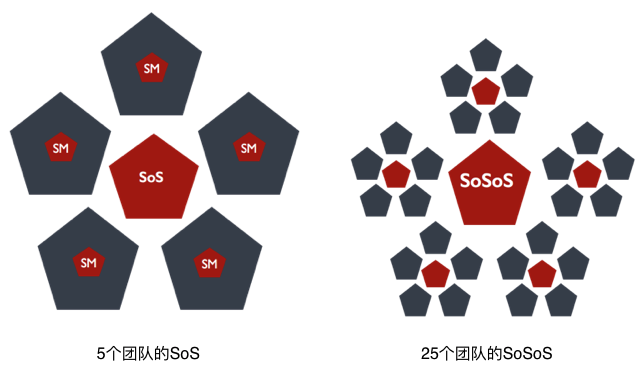
\includegraphics[width=1.0\linewidth]{Sos-R2.png}

\if0
\textbf{\textsc{note:}} While the Scrum Guide defines the optimal team size as being
3 to 9 people, Harvard research determined that optimal team size is 4.6
people.\footnote{Hackman, J Richard, Leading teams: Setting the stage for
great performances, Harvard Business Press, 2002} Experiments with high
performing Scrum teams have repeatedly shown that 4 or 5 people doing the
work is the optimal size. It is essential to linear scalability that this
pattern be the same for the number of teams in a SoS. Therefore, in the
above and following diagrams, pentagons were chosen to represent a team of
5. These diagrams are meant to be examples only, your organizational
diagram may differ greatly.
\fi
\textbf{\textsc{注意:}} スクラムガイドでは最適なチームサイズを3人から9人と定義しているが、ハーバードの調査では最適なチームサイズは4.6人であると判断されている。
\footnote{Hackman, J Richard, Leading teams: Setting the stage for great performances, Harvard Business Press, 2002} ハイパフォーマンスなスクラムチームにおける実験では、作業を行っている4人または5人が最適なサイズであることが繰り返し示されている。
このパターン、1つのSoS内のチーム数を同じにすることが、リニアなスケーラビリティにとって不可欠である。
したがって、上記および後の図では、5人のチームを表すために五角形としている。
これらの図は単なる例であり、実際の組織図は大きく異なる場合がある。

\if0
\subsection{The Executive Action Team}
\fi
\subsection{経営層上位レベルアクションチーム}
\if0
The Scrum of Scrums for the entire agile organization is called the
\textbf{Executive Action Team (EAT)}. The leadership team creates an agile bubble
in the organization where the Reference Model operates with 
its own guidelines and procedures that integrates effectively 
with any part of the organization that is not agile. It owns the agile ecosystem, 
implements the Scrum values, and assures that 
Scrum roles are created and supported.
\fi
アジャイル組織全体のスクラムオブスクラムは、\textbf{Executive Action Team (EAT)}と呼ばれる。
リーダーシップチームは、独自のガイドラインと手順によるリファレンスモデル運用により
組織で一つのアジャイルの泡を作る。それは、アジャイルではない組織のどのような部分
でも効果的に統合される。
アジャイルエコシステムを所有するということは、スクラムを実装し、スクラムのロールが
作成されサポートされていることを保証するということだ。

\if0
The EAT is the final stop for
impediments that cannot be removed by the SoS's that feed it. Therefore, it
must be comprised of individuals who are empowered, politically and
financially, to remove them. 
The function of the EAT is to coordinate
multiple SoS's (or SoSoS's) and to interface with any non-agile parts 
of the organization. As with any Scrum team, it needs a PO and SM.
It would be best if the EAT met daily as a Scrum team. They must meet at
least once per Sprint and have a transparent backlog.
\fi
EATは、SoSによって除去できない障害物に対する最終手段である。
したがって、それを除去するために政治的、経済的に権限を与えられた人物で構成されなければならない。
EATの機能は、複数のSoS(またはSoSoS)を調整することと、SoS内のチームの数
と同じである非アジャイル部分とのインタフェースすることである。
スクラムチームと同様に、POとSMが必要である。
EATは、スクラムチームとして毎日顔を合わせるのがベストかもしれない。
彼らはスプリントごとに少なくとも1回会合する必要があり、透明性のあるバックログを持ち合わせている
必要がある。

%\pagebreak
Sample Diagram showing an EAT coordinating 5 groupings of 25 teams:

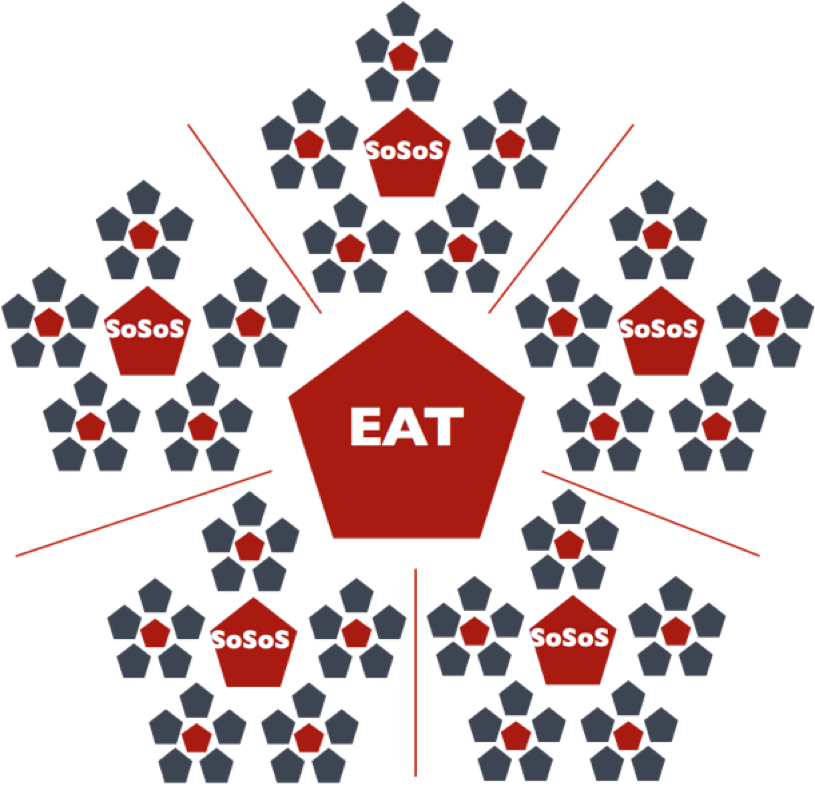
\includegraphics[width=\textwidth,height=\textheight,keepaspectratio]{SoS-EAT.png}

\if0
\subsection{The EAT's Backlog \& Responsibilities}
\fi
\subsection{EATのバックログと責務}
\if0
Scrum is an agile operating system that is different from traditional
project management. The entire SM organization reports into the EAT, which
is responsible for implementing this agile operating system by
establishing, maintaining, and enhancing the implementation in the
organization.
\fi
スクラムは、従来のプロジェクト管理とは異なるアジャイルな運用システムである。
SM組織全体はEATに対して報告を行う。これは、組織内で、このアジャイルな運用
システムを、確立、維持、実装強化することによって、実現するための責務である。
\if0
The EAT's role is to create an Organizational Transformation Backlog (a
prioritized list of the agile initiatives that need to be accomplished) and
see that it is carried out. For example, if there is a traditional Product
Development Life Cycle in the old organization, a new agile Product
Development Life Cycle needs to be created, implemented, and supported. It
will typically support quality and compliance issues better than the old
method but be implemented in a different way with different rules and
guidelines. The EAT ensures that a Product Owner organization is created and funded
and that this organization is represented on the EAT to support these efforts.
\fi
EATの役割は、組織変換バックログ(達成すべきアジャイルイニシアチブの優先順位
付けされたリスト)を作成し、それが実施されていることを確認することである。
たとえば、旧組織に伝統的な製品開発ライフサイクルが存在する場合、
新しいアジャイルな製品開発ライフサイクルを作成し、実装し、サポートする必要がある。
通常は、従来の方法よりも品質とコンプライアンスの問題をサポートするが、
異なるルールやガイドラインを使用し、異なる方法で実装する。
EATは、プロダクトオーナー組織が作成され、資金提供され、努力への支援表明を
保証する。

\if0
The EAT is accountable for the quality of Scrum within the organization.
Its responsibilities include but are not limited to:
\fi
EATは、組織内のスクラムの品質に責任を負う。
その責務には以下のものが含まれるが、これらに限定されることはない:
\if0
\begin{itemize}
\item creating an agile operating system for the Reference Model as it
scales through the organization, including corporate operational rules,
procedures, and guidelines to enable agility.
\item measuring and improving the quality of Scrum in the organization.
\item building capability within the organization for business agility.
\item creating a center for continuous learning for Scrum professionals.
\item supporting the exploration of new ways of working.
\end{itemize}
\fi
\begin{itemize}
\item 組織でスケール可能なリファレンスモデルのためのアジャイルな運用システムを作成する。それは、アジリティを得るための企業の運用ルール、手続き、ガイドラインを含む。
\item 組織でスクラムの品質を評価しカイゼンする
\item ビジネスにおけるアジリティのための組織力を構築する
\item スクラムのプロフェッショナルのための継続的学習のためのセンターを作成する
\item 新しい働き方の探求支援を行う
\end{itemize}
\if0
Finally, the EAT must set up and support a corresponding Product Owner
organization through associations of PO's that mirror the SoS's and scale
their PO functions. These teams of PO's and key stakeholders are known as
\textbf{MetaScrums}.
\fi
最後に、EATは、立ち上げ、PO間の協力によりSoSを反映したプロダクトオーナー組織の
サポート、PO機能をスケールさせることを行っていく必要がある。
これらのPOチームと主要ステークホルダーは、 \textbf{メタスクラム} として知られている。

\if0
\subsection{Outputs/Outcomes of the Scrum Master Cycle}
\fi
\subsection{スクラムマスターサイクルの出力と成果}
\if0
The SM organization (SoS, SoSoS, and EAT) work as a whole to complete the
other components of the Scrum Master Cycle: \textbf{Continuous Improvement
and Impediment Removal, Cross-Team Coordination, and Deployment}.

The goals of Continuous Improvement and Impediment Removal are to:
\fi
SM組織(SoS、SoSoS、およびEAT)は、スクラムマスターサイクルの他のコンポーネント、すなわち\textbf{継続的カイゼンと障害物の除去、チーム横断的な調整、および開発}を完了するために全体として機能する。

継続的カイゼンと障害物除去の目的は以下のとおり:
\if0
\begin{itemize}
\item identify impediments and reframe them as opportunities.
\item maintain a healthy and structured environment for prioritizing and
removing impediments, and then verifying the resulting improvements.
\item ensure visibility in the organization to effect change.
\end{itemize}
\fi
\begin{itemize}
\item 障害物を特定し視点を変える機会
\item 障害物の優先順位付けと除去のための健全かつ構造化された環境を維持する。また、その結果として得られるカイゼンを検証する
\item 効果的な変更のための組織における可視性を確保する
\end{itemize}
\if0
The goals of Cross-Team Coordination are to:
\begin{itemize}
\item coordinate similar processes across multiple related teams.
\item mitigate cross-team dependencies to ensure they don't become
impediments.
\item maintain alignment of team norms and guidelines for consistent output.
\end{itemize}
\fi
チーム横断的調整の目的は以下のとおり:
\begin{itemize}
\item 関連する複数のチーム間の同様のプロセスを調整する
\item チーム間のチーム横断的な依存関係を緩和し障害物とならないようにする
\item 一貫性のある出力のために、チームの規範とガイドラインの整合性を維持する
\end{itemize}

\if0
Since the goal of the SoS is to function as a release team, the deployment
of product falls under their scope, while what is contained in any release
falls under the scope of the Product Owners. Therefore, the goals of the
Deployment are to:
\begin{itemize}
\item deliver a consistent flow of valuable finished product to customers.
\item integrate the work of different teams into one seamless product.
\item ensure high quality of the customer experience.
\end{itemize}
\fi
SoSの目的はリリースチームとして機能することであり、プロダクトのデプロイメントはであり、何がリリースに含まれているかはプロダクトオーナーの範疇である。
したがって、(SoSの)デプロイメントの目的は次のとおり:
\begin{itemize}
\item 価値ある完成品の一貫した流れを顧客に届ける
\item 異なるチームの作業をシームレスな一つの製品に統合する
\item 高品質な顧客経験を確保する
\end{itemize}

\if0
\section{Product Owner Cycle}
\fi
\section{プロダクトオーナーサイクル}
\if0
\subsection{Coordinating the ``What'' - The MetaScrum}
A group of Product Owners who need to coordinate a shared backlog that
feeds a network of teams are themselves a team called a \textbf{MetaScrum}.
For each SoS there is an associated MetaScrum. A MetaScrum aligns the
teams' priorities along a single path so that they can coordinate their
team backlogs and build alignment with stakeholders to support the backlog.
A team's product owner is accountable for the composition and prioritization
of the team backlog and may pull backlog from the shared metascrum backlog
into the team backlog or generate independent backlog at his or her discretion.

MetaScrums hold a scaled version of Backlog Refinement, the \textbf{Scaled Backlog Refinement Meeting} 
\fi
\subsection{``What''を調整する - メタスクラム}
チームネットワークへのフィードバックとして共有バックログを調整する必要のあるプロダクトオーナーのグループ、それ自体が\textbf{メタスクラム}と呼ばれるチームである。
SoS毎に対応するメタスクラムがある。
メタスクラムは、チームの優先順位を一直線に調整しつつ、チームのバックログを調整し、ステークホルダーがバックログをサポートできるように連携を構築する。
ある1チームのプロダクトオーナーは、自チームのバックログの構成と優先順位付けの責務があり、共有メタスクラムバックログから自チームのバックログにバックログを引き出したり、自身の裁量で独自のバックログを生成したりする。

メタスクラムには、スケール化されたバックログリファインメントがある、\textbf{スケール化バックログリファインメントミーティング}である。
\if0
\begin{itemize}
\item Each team PO (or proxy) must attend
\item This event is the forum for Leadership, Stakeholders, or other
Customers to express their preferences
\end{itemize}
\fi
\begin{itemize}
\item 各チームのPO(または代理人)の出席は必須
\item このイベントは、リーダーシップ、ステークホルダーのための会である。または、顧客が自身の意見を表現する
\end{itemize}
\if0
This event occurs as often as needed, at least once per Sprint, to ensure a
Ready backlog. 

The main functions of the MetaScrum are to:
\begin{itemize}
\item create an overarching vision for the product \& make it visible to
the organization.
\item build alignment with key stakeholders to secure support for backlog
implementation.
\item generate a single, prioritized backlog; ensuring that duplication of
work is avoided.
\item create a minimally uniform ``Definition of Done'' that applies to all teams in
the SoS.
\item eliminate dependencies raised by the SoS.
\item generate a coordinated Release Plan.
\item decide upon and monitor metrics that give insight into the product.
\end{itemize}
\fi
このイベントは、バックログを準備完了にするため、スプリントごとに少なくとも1回、必要に応じて頻繁に行う。

メタスクラムの主たる機能はは以下のとおり:
\begin{itemize}
\item 製品の全体像を可視化し、組織に見えるようにする
\item バックログの実装の安全なサポートを確保するために主要なステークホルダーとの連携を構築する
\item 唯一の優先順位付けられたバックログを生成することで、作業の重複を避けることができる
\item SoSのすべてのチームに適用させる最小限で統一的な ``Doneの定義'' を作成する
\item SoSが提起した依存関係を排除する
\item 調整されたリリースプランを生成する
\item 製品への洞察力を与えるメトリクスを決定し監視する
\end{itemize}
\if0
MetaScrums, just like SoS's, function as Scrum teams on their own. As such,
they need to have someone who acts as a SM and keeps the team on track in
discussions. They also need a single person who is responsible for coordinating the
generation of a single Product Backlog for all of the teams covered by the
MetaScrum. This person is designated as the \textbf{Chief Product Owner}.

\subsection{The Chief Product Owner (CPO)}
\fi
SoSのように、メタスクラムは自立したスクラムチームとして機能します。
したがって、チーム内の議論を順調に進めさせれ、SMとして振る舞うことのできる誰かが必要となる。
また、メタスクラムがカバーするすべてのチームのための唯一のプロダクトバックログ生成を調整する責務を負う、たった一人の人物が必要である。
この人物は、\textbf{チーフプロダクトオーナー}に指定される。

\subsection{チーフプロダクトオーナー (CPO)}
\if0
Through the MetaScrums, Chief Product Owners coordinate priorities among
Product Owners who work with individual teams. They align backlog
priorities with Stakeholder and Customer needs. Just like a SoSM, they may
be an individual team PO who chooses to play this role as well, or they may
be a person specifically dedicated to this role. Their main
responsibilities are the same as a regular PO's, but at scale:
\begin{itemize}
\item Setting a strategic vision for the whole product.
\item Creating a single, prioritized backlog of value to be delivered by
all of the teams.
\begin{itemize}
\item these items would be larger Product Backlog Items than that for a team PO.
\end{itemize}
\item Working closely with their associated SoSM so that the Release Plan
that the MetaScrum team generates can be deployed efficiently.
\item Monitoring customer product feedback and adjusting the backlog
accordingly.
\end{itemize}
\fi
チーフプロダクトオーナーは、メタスクラムを通じて、個々のチームで働くプロダクトオーナー間の優先順位を調整する。
ステークホルダーおよび顧客ニーズに合わせ、バックログの優先順位を調整する。
SoSMのように、この役割を果たすことを選択した個別チームのPOである場合もあれば、この役割に特化した個人の場合もある。
彼らの主な責務は通常のPOと同じである。しかしスケール化では:
\begin{itemize}
\item 製品全体の戦略的ビジョンを設定する
\item 全チームに配布する、価値により優先順位付けされた唯一のバックログを作成する
\begin{itemize}
\item これらのアイテムは、チームPOのものよりも大きなプロダクトバックログアイテムとなる
\end{itemize}
\item 効率的なデプロイのためにメタスクラムチームが生成するリリースプランのために、関連するSoSMと緊密に連携する
\item 顧客プロダクトのフィードバックを監視し、それに応じてバックログを調整する
\end{itemize}

\if0
\subsection{Scaling the MetaScrum}
Just as SoS's can grow into SoSoS's, MetaScrums can also expand by the same
mechanism. There is no specific term associated with these expanded units,
nor do the CPO's of them have specific expanded titles. We encourage each
organization to develop their own. For the following diagrams, we have
chosen to add an additional ``Chief'' to the title of those PO's as they
magnify out.
\fi
\subsection{メタスクラムのスケーリング}
SoSがSoSoSへ拡張可能なのと同様に、メタスクラムも同じメカニズムで拡張する。
これらの拡張ユニットには特定の用語はなく、CPOの特定の拡張された肩書もない。
これは、各組織で独自開発することを奨励する。
以下の図では、拡大されたPOの肩書に``チーフ''を追加することにしている。

%\pagebreak
\if0
Some sample diagrams:
\fi
参考図:

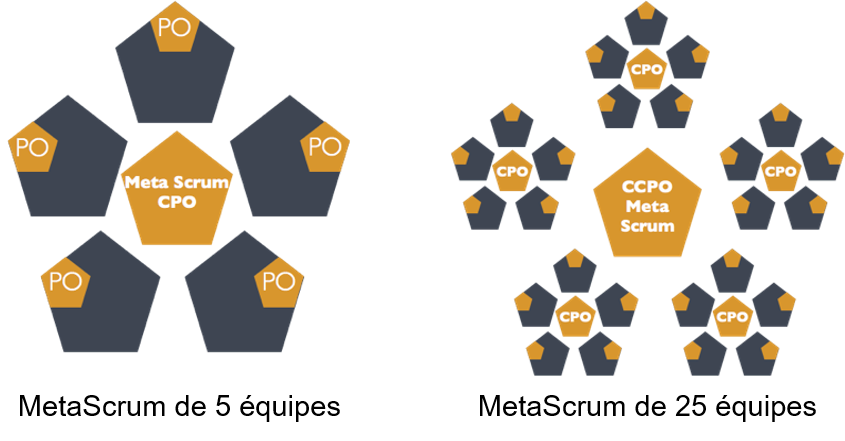
\includegraphics[width=1.0\linewidth]{MetaScrum-R2.png}

\if0
\textbf{NOTE:} As mentioned above, these pentagons represent the ideal
sized Scrum teams and ideal sized MetaScrums. These diagrams are meant to
be examples only, your organizational diagram may differ greatly.
\fi
\textbf{注意:} 上記は、五角形は、理想サイズのスクラムチームと理想サイズのメタスクラムを表している。
これらの図は単なる例であり、あなたの組織図では大きく異なる場合がある。

\if0
\subsection{The Executive MetaScrum (EMS)}
The MetaScrums enable a network design of Product Owners which is
infinitely scalable alongside their associated SoS's. The MetaScrum for the
entire agile organization is the \textbf{Executive MetaScrum}. The EMS owns
the organizational vision and sets the strategic priorities for the whole
company, aligning all the teams around common goals.
\fi
\subsection{エグゼクティブメタスクラム (EMS)}
メタスクラムは、関連するSoSとともに、無限にスケール可能なプロダクトオーナーのネットワークデザインを可能にする
アジャイル組織全体のメタスクラムは\textbf{エグゼクティブメタスクラム}である。
EMSは、組織のビジョンを持ち、共通の目的に沿ってすべてのチームを調整しながら、会社全体の戦略的な優先事項を設定します。

\if0
Sample diagram showing an EMS coordinating 5 groups of 25 teams:
\fi
25チームの5つのグループを調整するEMSを示す参考図:

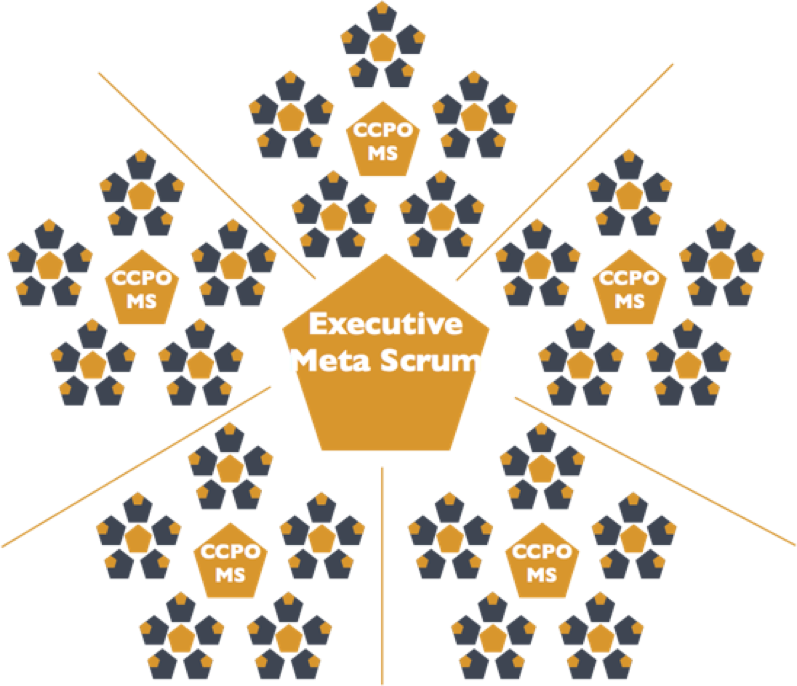
\includegraphics[width=1.0\linewidth]{ExecMetaScrum.png}

\if0
\subsection{Outputs/Outcomes of the Product Owner Organization}
The PO organization (various MetaScrums, the CPO's, and the Executive
MetaScrum) work as a whole to satisfy the components of the Product Owner
Cycle: \textbf{Strategic Vision, Backlog Prioritization, Backlog
Decomposition \& Refinement, and Release Planning}.

The goals of setting a Strategic Vision are to:
\fi
\subsection{プロダクトオーナー組織の出力と成果}
PO組織(多様なメタスクラム、CPO、エグゼクティブメタスクラム)は、プロダクトオーナーサイクル:
\textbf{戦略的ビジョン、バックログ優先順位付け、バックログ分解とリファインメント、リリースプランニング}の全体を満足させるための構成要素として機能する。

戦略的ビジョンを設定する目的は以下のとおり:
\if0
\begin{itemize}
\item clearly align the entire organization along a shared path forward.
\item compellingly articulate why the organization exists.
\item describe what the organization will do to leverage key assets in
support of its mission.
\item respond to rapidly changing market conditions.
\end{itemize}
\fi
\begin{itemize}
\item 組織全体を共有済みの進行経路に沿って明確に整列させる
\item 組織の存在意義を説得力を以て明確にする
\item ミッションにおいてキーとなる資産を活用するために組織が何をすべきかについて説明する
\item 急速に変化するマーケットの状況に対応する
\end{itemize}
\if0
The goals of Backlog Prioritization are to:
\begin{itemize}
\item identify a clear ordering for products, features, and services to be
delivered.
\item reflect value creation, risk mitigation and internal dependencies in
ordering of the backlog.
\item prioritize the high-level initiatives across the entire agile
organization prior to Backlog Decomposition and Refinement.
\end{itemize}
\fi
バックログ優先順位付けの目的は以下のとおり:
\begin{itemize}
\item デリバリする製品、機能、サービスの注文を明確に識別する
\item バックログの順序付けにおける価値創造、リスク軽減、内部依存関係を反映する
\item バックログの分解とリファインメントに先立ち、アジャイル組織全体のハイレベルイニシアチブを優先する
\end{itemize}
\if0
The goals of Backlog Decomposition \& Refinement are to:
\begin{itemize}
\item break complex products and projects into independent functional
elements that can be completed by one team in one Sprint.
\item capture and distill emerging requirements and customer feedback.
\item ensure all backlog items are truly ``Ready'' so that they can be
pulled by the individual teams.
\end{itemize}
\fi
バックログ分解とリファインメントの目的は以下のとおり:
\begin{itemize}
\item 複雑な製品やプロジェクトを、1つのチーム1つのスプリントで完成させることができる独立した機能要素に分割する
\item 新たな要件と顧客からのフィードバックを収集し、抽出する
\item すべてのバックログアイテムが本当に ``Ready'' であることを確認して、個々のチームが引き取れるようにする
\end{itemize}
\if0
The goals of Release Planning are to:
\begin{itemize}
\item forecast delivery of key features and capabilities.
\item communicate delivery expectations to stakeholders.
\item update prioritization, as needed.
\end{itemize}
\fi
リリースプランニングの目的は以下のとおり:
\begin{itemize}
\item 主要機能のデリバリ予測
\item ステークホルダーへ納期を伝える
\item 必要に応じて優先順位を更新する
\end{itemize}

\if0
\section{Connecting the PO/SM Cycles}
\fi
\section{PO/SM サイクルの接続}

\if0
\subsection{Understanding Feedback}
The \textbf{Feedback} component is the second point where the PO \& SM
Cycles touch. Product feedback drives continuous improvement through
adjusting the Product Backlog while Release feedback drives continuous
improvement through adjusting the Deployment mechanisms. The goals of
obtaining and analyzing Feedback are to:
\fi
\subsection{フィードバックを理解する}
\textbf{フィードバック}コンポーネントは、POとSMサイクルが接触する2番目のポイントである。
プロダクトフィードバックは、プロダクトバックログの調整を通じて継続的改良を推進し、同時に、リリースフィードバックが、デプロイメカニズムの調整を通じて継続的カイゼンを推進する。
フィードバックの取得と分析の目的は以下の通り:
\if0
\begin{itemize}
\item validate our assumptions.
\item understand how customers use and interact with the product.
\item capture ideas for new features and functionality.
\item define improvements to existing functionality.
\item update progress towards product/project completion to refine release
planning and stakeholder alignment.
\item identify improvements to deployment methods and mechanisms.
\end{itemize}
\fi
\begin{itemize}
\item 自分たちの仮説を検証する
\item 顧客がプロダクトをどのように使用し、相互作用するかを理解する
\item 新しい機能や機能性のアイデアを収集する
\item 既存の機能の改良を定義する
\item リリース計画とステークホルダー整合性をカイゼンするために、製品/プロジェクト完了までの進捗状況を更新する
\item デプロイ方法と仕組みのカイゼンを識別する
\end{itemize}

\if0
\subsection{Metrics \& Transparency}
Radical transparency is essential for Scrum to function optimally, but it
is only possible in an organization that has embraced the Scrum values. It
gives the organization the ability to honestly assess its progress and to
inspect and adapt its products and processes. This is the foundation of the
empirical nature of Scrum as laid out in the Scrum Guide.

Both the SM \& PO Cycles require metrics that will be decided upon by the
separate SM and PO organizations. Metrics may be unique to both specific
organizations as well as to specific functions within those organizations.
Scrum@Scale does not require any specific set of metrics, but it does
suggest that at a bare minimum, the organization should measure:
\fi
\subsection{メトリクスと透明性}
スクラムが最適に機能するために、根本的な透明性が不可欠であり、スクラムの価値を抱擁した組織でのみ可能となる。
これは、組織に、誠実な進捗状況アクセス、製品とプロセスを検査、適応させる能力を組織に与える。
これは、スクラムガイドで示されているスクラムの経験的性質の基礎となっている。

SMとPOサイクル双方において、SMとPO分離組織によって決定されるメトリクスを必要とする。
メトリクスは、特定組織だけでなく、それらの組織内の特定機能にも固有となるであろう。
Scrum@Scaleは特定のメトリクスセットを必要としていないが、最低限のものについて示す。組織が計測すべきものは以下である:
\if0
\begin{itemize}
\item Productivity - e.g. change in amount of Working Product delivered per
Sprint
\item Value Delivery - e.g. business value per unit of team effort
\item Quality - e.g. defect rate or service downtime
\item Sustainability - e.g. team happiness
\end{itemize}
\fi
\begin{itemize}
\item 生産性 - e.g. スプリントごとに届けられるプロダクトの作業量の変化
\item 価値のデリバリ - e.g. チームの労力あたりのビジネス価値
\item 品質 - e.g. 不具合率またはサービス停止時間
\item 持続可能性 - e.g. チームの幸福
\end{itemize}
\if0
The goals of having Metrics and Transparency are to:
\begin{itemize}
  \item provide all decision makers, including team members, with
appropriate context to make good decisions.
\item shorten feedback cycles as much as possible to avoid over-correction.
\item require minimal additional effort by teams, stakeholders or
leadership.
 \end{itemize}
\fi
メトリクスと透明性を持つことの目的は以下のおとり:
\begin{itemize}
  \item チームメンバーを含むすべての意思決定者に、適切な判断を下すための適切なコンテキストを提供する
\item 過剰な是正を避けるためにフィードバックサイクルをできるだけ短くする
\item チーム、ステークホルダー、リーダーシップによる最小限の努力を要求する
 \end{itemize}

\if0
\subsection{Some notes on Organizational Design}
The scale-free nature of Scrum@Scale allows the design of the organization
to be component-based, just like the framework itself. This permits for
rebalancing or refactoring of teams in response to the market. As an
organization grows, capturing the benefits of distributed teams may be
important. Some organizations reach talent otherwise unavailable and are
able to expand and contract as needed through outsourced development.
Scrum@Scale shows how to do this while avoiding long lag times, compromised
communications, and inferior quality, enabling linear scalability both in
size and global distribution.\footnote{Sutherland, Jeff and Schoonheim,
Guido and Rustenburg, Eelco and Rijk, Maurits, ``Fully distributed scrum:
The secret sauce for hyperproductive offshored development teams'',
AGILE'08. Conference, IEEE: 339-344, 2008}
\fi
\subsection{組織デザインにおける考慮点}
Scrum@Scaleのスケールフリーの性質により、フレームワーク自体と同様に、組織の設計をコンポーネントベースにすることができる。
これにより、マーケットに応じてチームのリバランスやリファクタリングが可能となる。
組織が成長するにつれて、分散チームのメリットを得ることが重要となるであろう。
一部の組織では、他には利用できない才能があり、アウトソーシング開発を通じて、必要に応じて拡大したり縮小することができる。
Scrum@Scaleは、長いラグタイム、コミュニケーション妥協、品質劣化を避けながら、これを行う方法を示し、サイズとグローバル分散の両方でリニアなスケーラビリティを実現する。
\footnote{Sutherland, Jeff and Schoonheim,
Guido and Rustenburg, Eelco and Rijk, Maurits, ``Fully distributed scrum:
The secret sauce for hyperproductive offshored development teams'',
AGILE'08. Conference, IEEE: 339-344, 2008}

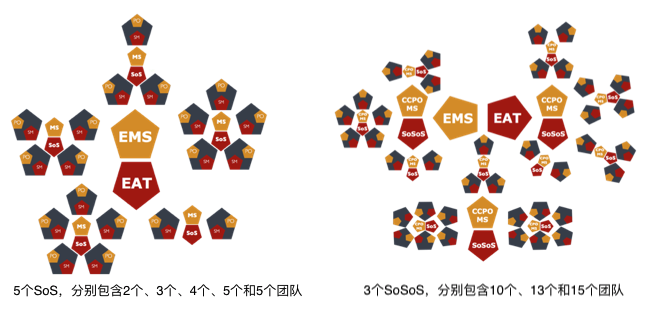
\includegraphics[width=1.0\linewidth]{VariableSoS-R2.png}
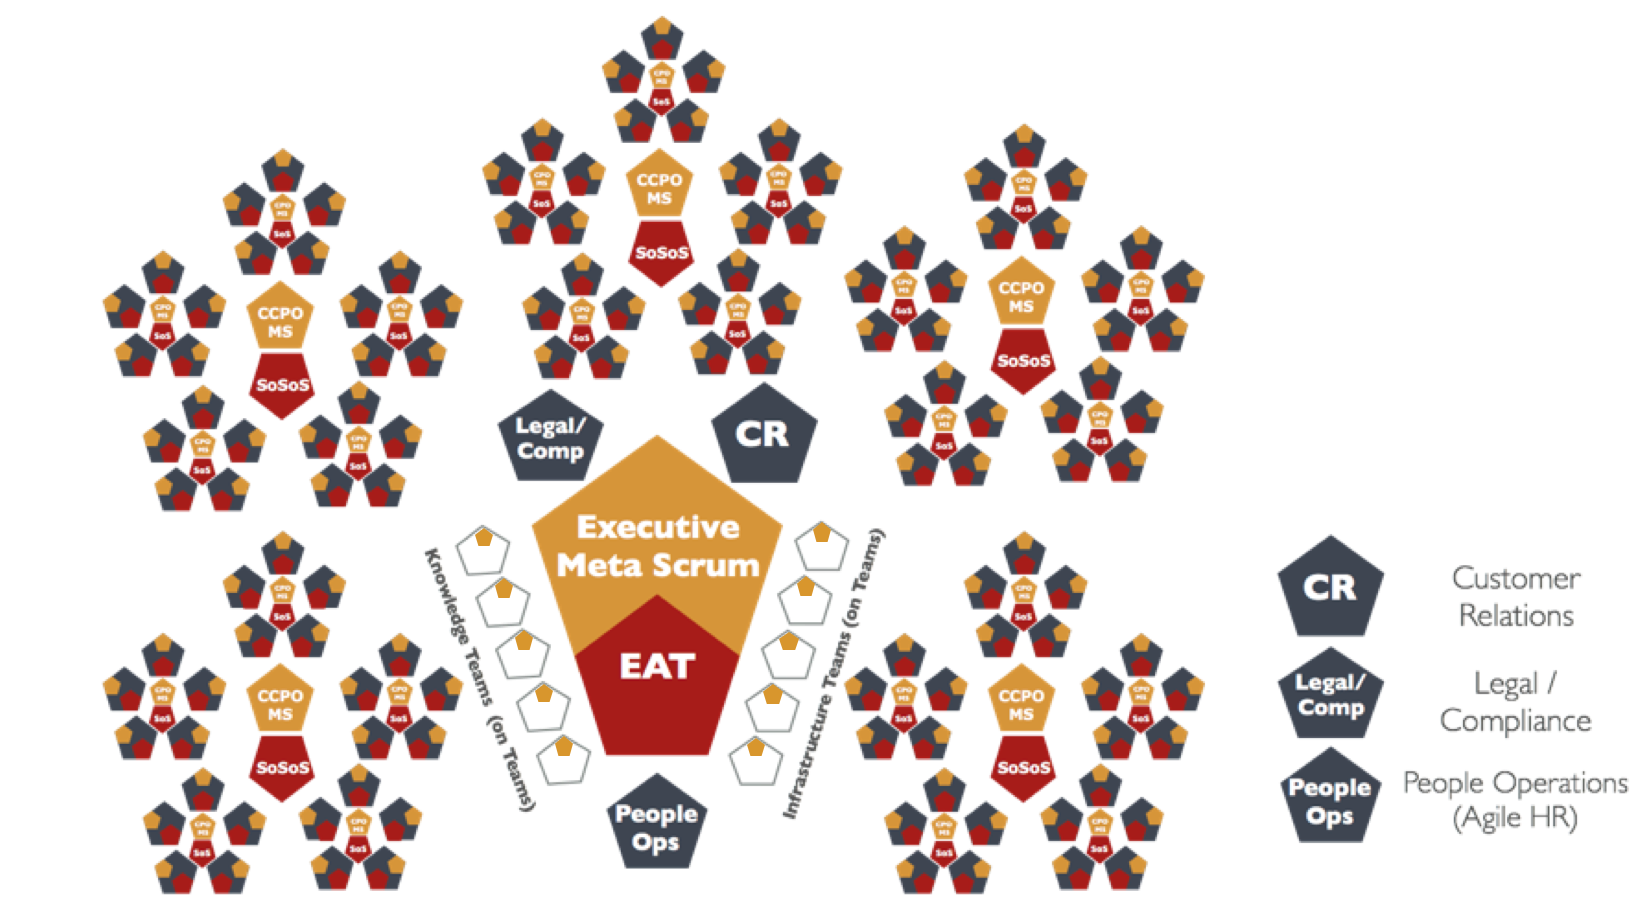
\includegraphics[width=1.0\linewidth]{OrganizationalDiagram.png}

\if0
In this organizational diagram, the \textbf{Knowledge \& Infrastructure
Teams} represent virtual teams of specialists of which there are too few to
staff each team. They coordinate with the Scrum teams as a group via
service-level agreements where requests flow through a PO for each
specialty who converts them into a transparent ordered backlog. An
important note is that these teams are NOT silos of individuals who sit
together (this is why they are represented as hollow pentagons); their team
members sit on the actual Scrum teams, but they make up this virtual Scrum
of their own for the purpose of backlog dissemination and process
improvement.

\textbf{Customer Relations, Legal / Compliance, and People Operations} are
included here since they are necessary parts of organizations and will
exist as independent Scrum teams on their own, which all of the others may
rely upon.

A final note on the representation of the EAT \& EMS: in this diagram, they
are shown as overlapping since some members sit on both of the teams. In very
small organizations or implementations, the EAT \& EMS may consist entirely
of the same team members.
\fi
この組織図では、\textbf{ナレッジ \& インフラストラクチャチーム}が、各チームのスタッフが非常に少ない専門家の仮想チームを表している。
彼らはスクラムチームとSLAを結ぶグループとして調整を行い、要求は、透明性をもつ優先順位付けされたバックログへ変換を行う各専門分野ごとのPOを通じて流れる。
重要な点は、これらのチームが一緒に座っている個人のサイロではないということである(白抜き五角形で表されている理由)。
彼らのチームメンバーは実際のスクラムチームに座っているが、バックログ配布とプロセスカイゼンのために、この仮想スクラムを構成する

\textbf{顧客関係、法務/コンプライアンス、および人事部門}は、組織の必要な部分であり、他のすべてが頼る独立したスクラムチームとして存在するため、ここに含まれている。

EAT \& EMSの表現に関する最後の注記: この図では、一部のメンバーが両方のチームに在席しているため、重複して表現している。
非常に小規模な組織や実装では、EATとEMSはまったく同じチームメンバーで構成されている場合がある。

\if0
\section{End Note}
Scrum@Scale is designed to scale productivity, to get the entire
organization doing twice the work in half the time with higher quality and
in a significantly improved work environment. Large organizations that
properly implement the framework can cut the cost of their products and
services while improving quality and innovation.

Scrum@Scale is designed to saturate an organization with Scrum. All teams,
including Leadership, Human Resources, Legal, Consulting \& Training, and
product \& service teams, implement the same style of Scrum while
streamlining and enhancing an organization.

Well implemented Scrum can run an entire organization.
\fi
\section{後書}
Scrum@Scaleは生産性を向上させ、組織全体を高品質で大幅にカイゼンされた作業環境で半分の時間で2倍の作業を行うように設計されている。
このフレームワークを適切に実装している大規模な組織は、品質と革新性を向上させながら、製品とサービスのコストを削減している。

Scrum@Scaleは、組織にスクラムで浸透させるように設計されている。
リーダーシップ、人事、法務、コンサルティング \& トレーニング、製品 \& サービスチームを含むすべてのチームで、
組織の合理化と強化を行うと同時に同じスタイルのスクラムを実装する。

うまく実装されたスクラムにより、組織全体を運営することができる。
\if0
\section{Acknowledgements}
We acknowledge IDX for the creation of the Scrum of Scrums which first
allowed Scrum to scale to hundreds of teams,\footnote{Sutherland, Jeff,
``Inventing and Reinventing SCRUM in five Companies'', Sur le site officiel
de l'alliance agile, 2001} PatientKeeper for the creation of the
MetaScrum,\footnote{Sutherland, Jeff, ``Future of scrum: Parallel pipelining
of sprints in complex projects'', Proceedings of the Agile Development
Conference,  IEEE Computer Society 90-102,  2005.} which enabled rapid
deployment of innovative product, and OpenView Venture Partners for scaling
Scrum to the entire organization.\footnote{Sutherland, Jeff and Altman,
Igor, ``Take no prisoners: How a venture capital group does scrum'', Agile
Conference, 2009. AGILE'09, IEEE 350-355.  2009} We value input from Intel
with over 25,000 people doing Scrum who taught us ``nothing scales'' except
a scale-free architecture, and SAP with the largest Scrum team product
organization who taught us management involvement in the MetaScrum is
essential to get 2,000 Scrum teams to work together.

The agile coaches and trainers implementing these concepts at Amazon, GE,
3M, Toyota, Spotify, Maersk, Comcast, AT\&T and many other companies working with Jeff Sutherland
have been helpful in testing these concepts across a wide range of
companies in different domains.

And finally, Avi Schneier and Alex Sutherland have been invaluable in
formulating and editing this document.
\fi
\section{謝辞}
我々は、IDX社において、スクラムを何百ものチームに広げることを最初に許してくれたことで、スクラムオブスクラムが作成できたと認識している。
\footnote{Sutherland, Jeff, ``Inventing and Reinventing SCRUM in five Companies'', Sur le site officiel de l'alliance agile, 2001} 
PentientKeeper社ではメタスクラムを作成し、
\footnote{Sutherland, Jeff, ``Future of scrum: Parallel pipelining of sprints in complex projects'', Proceedings of the Agile Development Conference,  IEEE Computer Society 90-102,  2005.} 
革新的な製品の高速開発を可能にし、OpenView Venture Partnersはスクラムを組織全体に拡大した。
\footnote{Sutherland, Jeff and Altman, Igor, ``Take no prisoners: How a venture capital group does scrum'', Agile Conference, 2009. AGILE'09, IEEE 350-355.  2009} 
Intel社の25,000人以上によるスクラムの実践は、スケールフリーアーキテクチャ無しには``何もスケールない''ことを私たちに教え、
最大のスクラムチーム製品部門を持つSAP社は、2,000のスクラムチームがともに働くためには、メタスクラムにおけるマネジメントの関与が必須であるということを教えてくれた。

Amazon, GE, 3M, Toyota, Spotify, Maersk, Comcast, AT\&Tと多くの企業で
Jeff Sutherlandとこれらのコンセプトを実装のために働いてくれているアジャイルコーチとトレーナーたちは、
異なるドメインの幅広い企業をまたがりこれらコンセプトをテストすることに役立ち続けてくれている。

最後に、Avi SchneierとAlex Sutherlandは、この文書の作成と編集において非常に貴重な存在である。

\pagebreak

\printbibliography



\end{document}
